Unix provides several solutions to perform \gls{ipc}. Sockets use file descriptors to fulfill this task. This section introduces relevant details regarding both internet sockets and local (Unix domain) sockets focusing on the stream socket type. Also, sockets are handled differently regarding the virtual memory of the system: user space and kernel space. Firstly we'll present a simple server-client model implementation at user space followed by some particularities of socket implementation at kernel level.

\subsection{Stream Sockets}

Unix systems provide a programming interface to easily carry out \gls{ipc} tasks using sockets. This \gls{api} is present in the \texttt{sys/socket.h} header file. Sockets follow a server-client based model, in which a sequence of primitives needs to be invoked in order to established the connection. This sequence depends on the protocol that will take place. Usually, sockets fall into the \gls{tcp} or \gls{udp} protocols. Both require different primitives to settle connections. In the scope of this project, only stream sockets are used. Therefore, this section will focus on the basic behavior of stream sockets. \autoref{fig:server_client_sockets} illustrates a typical case and may be described as follows:

\begin{figure}[h]
 \centering
 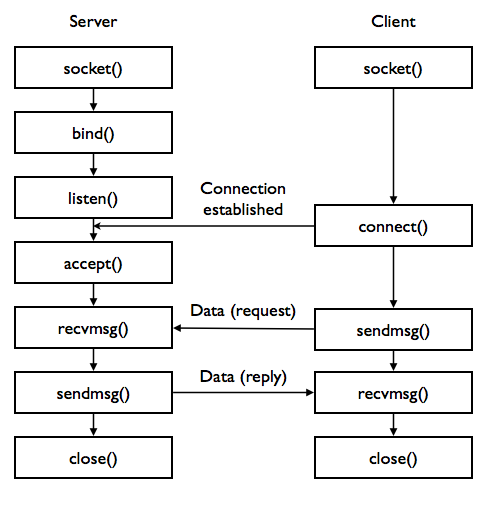
\includegraphics[scale=0.5]{figures/server_client_sockets.png}
 \caption{Typical server-client based model of stream sockets}
 \label{fig:server_client_sockets}
\end{figure}

\begin{enumerate}
\item The server initializes the process by creating a file descriptor (socket descriptor). This process is accomplished through the \texttt{socket()} primitive:

\begin{lstlisting}[caption=Declaration of the \texttt{socket()} function]
int socket(int domain, int type, int protocol);
\end{lstlisting}

The returned value defines the socket descriptor. As arguments, \textit{domain} specifies the socket family (\texttt{AF\_INET}, \texttt{AF\_INET6}, \texttt{AF\_UNIX}, etc), \textit{type} specifies the socket type (\texttt{SOCK\_DGRAM}, \texttt{SOCK\_STREAM}, etc) and \textit{protocol} indicates a particular protocol to be used with the socket, but usually takes the value 0.

\item Once created, the socket is unnamed and needs to be bound to an address in order to be identified by the system. This address will be assigned depending on the socket family. The \texttt{bind()} primitive is presented as follows:

\begin{lstlisting}[caption=Declaration of the \texttt{bind()} function]
int bind(int socket, const struct sockaddr *address, socklen_t address_len);
\end{lstlisting}

If the returned value is 0, the operation was successful. In case of error, returns -1. The argument \textit{socket} specifies the socket descriptor previously created, the \textit{address} points to the address to be bound to the socket and \textit{address\_len} indicates the length of the address structure.

\item After the binding, the server is ready to establish a connection to a client. Thus, the server is kept listening to connection requests through \texttt{listen()}:

\begin{lstlisting}[caption= Declaration of the \texttt{listen()} function]
int listen(int socket, int backlog);
\end{lstlisting}

The function expresses the success or failure of the operation through the returned value, being 0 or -1, respectively. It takes as arguments the file descriptor and a \textit{backlog} that defines the length of the socket's listen queue, where connection requests are stored.

\item At this point, the server is waiting for some request from a client. To set up a client socket, primarily it is executed the \texttt{socket()} primitive to create a file descriptor.

\item Once the socket descriptor is created, the client must specify the server address to get connected. The \texttt{connect()} primitive is used:

\begin{lstlisting}[caption=Declaration of the \texttt{connect()} function]
int connect(int socket, const struct sockaddr *address, socklen_t address_len);
\end{lstlisting}

It returns 0 on success or -1 on error. The \textit{socket} indicates the client socket descriptor, the \textit{address} points to the server address and \textit{address\_len} defines the length of the address.

\item The server receives the connection request and is able to accept it through the \texttt{accept()} primitive:

\begin{lstlisting}[caption=Declaration of the \texttt{accept()} function]
int accept (int socket, struct sockaddr *address, socklen_t *address_len);
\end{lstlisting}

This primitive returns a newly connected socket descriptor. The \textit{address} is filled with the address of the client and \textit{address\_len} defines the length of this address. Both sockets are ready to start the communication.

\item The client and server may exchange data through some primitives. In this case, we'll introduce \texttt{sendmsg()} and \texttt{recvmsg()}:

\begin{lstlisting}[caption=Declaration of the \texttt{sendmsg()} and \texttt{recvmsg()} function]
ssize_t sendmsg (int socket, const struct msghdr *message, int flags);

ssize_t recvmsg(int socket, struct msghdr *message, int flags);
\end{lstlisting}

These primitives use a special structure to store data in the \textit{message} argument, that is the \texttt{struct msghdr}. Further in this section we'll inspect this structure. The \textit{flags} argument specifies some conditions such as, for instance, blocking the function until the total amount of data requested is returned, by the flag \texttt{MSG\_WAITALL}. The total amount of data exchanged is stored on the returned value.

\item At last, when all data has been exchanged both sockets need to close its connections by calling the \texttt{close()} primitive:

\begin{lstlisting}[caption=Declaration of the \texttt{close()} function]
int close(int fildes);
\end{lstlisting}

The socket descriptor is passed as argument.
\end{enumerate}

\subsection{Address Formats}

As previously mentioned, in the primitives \texttt{bind()}, \texttt{connect()} and \texttt{accept()} the argument \textit{address} points to a \texttt{sockaddr} structure based on the socket's family. If we want to communicate through internet sockets, the family is defined as \texttt{AF\_INET} or \texttt{AF\_INET6}, depending on the \gls{ip} version, IPv4 or IPv6, respectively, and a \texttt{sockaddr\_in} or \texttt{sockaddr\_in6} structure is used to handle internet addresses:

\begin{lstlisting}[caption=Declaration of the \texttt{sockaddr\_in} structure]
struct sockaddr_in {
    short			sin_family; 
    unsigned short	sin_port;
    struct in_addr	sin_addr; 
    char			sin_zero[8]; 
}
\end{lstlisting}

This structure defines the required data to create an internet address: the port and the \gls{ip} address \cite{IPSockets:Beej}. These fields are specified by \texttt{sin\_port} and \texttt{sin\_addr}, respectively. The former is stored as an \texttt{unsigned short}. The last is defined by a \texttt{in\_addr} structure that contains an \texttt{unsigned long} to store the \gls{ip} address value:

\begin{lstlisting}[caption=Declaration of the \texttt{in\_addr} structure]
struct in_addr {
    unsigned long s_addr;
}
\end{lstlisting}

When it concerns the \texttt{AF\_INET6} family, sockets use the \texttt{sockaddr\_in6} structure:

\begin{lstlisting}[caption=Declaration of the \texttt{sockaddr\_in} structure]
struct sockaddr_in6 {
    sa_family_t     sin6_family;
    in_port_t       sin6_port;
    uint32_t        sin6_flowinfo;
    struct in6_addr sin6_addr;
    uint32_t        sin6_scope_id;
}
\end{lstlisting}

The element \texttt{sin6\_family} is defined by the \texttt{AF\_INET6} macro, the \texttt{sin6\_port} specifies the protocol port, \texttt{sin6\_flowinfo} and \texttt{sin6\_scope\_id} characterize identifiers of the flow and the address, respectively and, at last, the \texttt{sin6\_addr} defines the \gls{ip} address through a \texttt{in6\_addr} structure. This structure presents an \texttt{unsigned char} array that stores the \gls{ip} address:

\begin{lstlisting}[caption=Declaration of the \texttt{in6\_addr} structure]
struct in6_addr {
    unsigned char   s6_addr[16];
}
\end{lstlisting}

These structures are declared in the \texttt{netinet/in.h} header file.

In local sockets the family is defined by \texttt{AF\_UNIX} and the address is set using a \texttt{sockaddr\_un} structure:

\begin{lstlisting}[caption=Declaration of the \texttt{sockaddr\_un} structure]
#define UNIX_PATH_MAX    108

struct sockaddr_un {
    sa_family_t	sun_family;
    char		sun_path[UNIX_PATH_MAX];
}
\end{lstlisting}

The address is defined by the path of a file stored in \texttt{sun\_path}. In the scope of this project, there are two types of paths (called namespaces) that are important to distinguish: 

\begin{itemize}
\item \textit{Pathname}: a null-terminated filesystem pathname is bound to the local socket.
\item \textit{Abstract}: the \texttt{sun\_path[0]} is a null byte. The socket's address in this namespace is given the additional bytes in \texttt{sun\_path}. The name has no connection to the filesystem pathnames\footnote{http://man7.org/linux/man-pages/man7/unix.7.html}.
\end{itemize} 

The \texttt{sockaddr\_un} structure is declared in the \texttt{sys/un.h} header file.

\subsection{Address Lookup}

Sockets store \gls{ip} addresses as \texttt{unsigned long}s or \texttt{unsigned char} arrays, but they are displayed to users through the dotted notation: \texttt{x.x.x.x} in case of \gls{ip}v4 or \texttt{x:x:x:x:x:x:x:x} in case of \gls{ip}v6. In order to translate internet socket addresses to the user's reading format, the \texttt{arpa/inet.h} header file provides the following function:

\begin{lstlisting}[caption=Declaration of the \texttt{inet\_ntop()} function]
const char *inet_ntop(int af, const void *restrict src, char *restrict dst, socklen_t size);
\end{lstlisting}

This function takes as arguments the internet family in \textit{af} (\texttt{AF\_INET} or \texttt{AF\_INET6}); \textit{src} points to a buffer holding a \texttt{struct in\_addr} or a \texttt{struct in6\_addr}; \textit{dst} points to the destination string and \textit{size} indicates the maximum length of this string.

Using internet addresses is also possible to get the both the host and service name through the \texttt{getnameinfo()} function, declared on the \texttt{netdb.h} header file:

\begin{lstlisting}[caption=Declaration of the \texttt{getnameinfo()} function]
int getnameinfo(const struct sockaddr *sa, socklen_t salen,
                char *host, size_t hostlen,
                char *serv, size_t servlen, int flags);
\end{lstlisting}


\subsection{Kernel Sockets}

In kernel space, the server-client based model is the same, but the primitives are different. In order to understand how socket primitives are handled in kernel space it was necessary to check the Linux Cross Reference\footnote{http://lxr.free-electrons.com}. Sockets are created through the \texttt{sock\_create()} primitive, declared in the \texttt{linux/net.h} header file:

\begin{lstlisting}[caption=Declaration of the \texttt{sock\_create()} function]
int sock_create(int family, int type, int proto, struct socket **res);
\end{lstlisting}

The first three arguments are similar to the \texttt{socket()} primitive described above. Kernel creates a socket by allocating memory to a \texttt{struct socket} and filling it in with the following data:

\begin{lstlisting}[caption=Declaration of the \texttt{socket} structure]
struct socket {
   socket_state state;
   short type;
   unsigned long flags;
   struct socket_wq __rcu  *wq;
   struct file * file;
   struct sock * sk;
   const struct proto_ops * ops;
}
\end{lstlisting}

From these structure's fields it is important to highlight the following: \textit{type} that indicates the socket type (\texttt{SOCK\_STREAM}, \texttt{SOCK\_DGRAM}, etc); \textit{sk} that specifies all internal networking protocol and is an agnostic socket representation, i. e. the same structure is used by any socket independently of its type or family; and \textit{ops} that defines the socket operations. Once the \texttt{sock\_create()} primitive is executed, the socket data is stored at \textit{res}.

This socket will execute the remaining operations through the \texttt{struct proto\_ops} presented in the \textt{struct socket} by means of \textit{ops} field:

\begin{lstlisting}[caption=Declaration of the \texttt{proto\_ops} structure]
struct proto_ops {
    int family;
    struct module   *owner;
    int (*release) (struct socket *sock);
    int (* bind) (struct socket *sock, struct sockaddr *myaddr, int sockaddr_len);
    int (* connect) (struct socket *sock, struct sockaddr *vaddr, int sockaddr_len, int flags);
    int (* accept) (struct socket *sock, struct socket *newsock, int flags);
    int (* listen) (struct socket *sock, int len);
(...)
}
\end{lstlisting}

All primitives, \texttt{bind()}, \texttt{connect()}, \texttt{listen()}, \texttt{accept()}, and \texttt{release()}, which is the kernel implementation of \texttt{close()}, are called through this structure that belongs to the socket. They are the kernel implementation of those forementioned primitives in user space and take almost the same arguments, but instead of using the socket descriptor, they point to the socket structure in \textit{sock}.

To send and receive data, kernel declares the \texttt{sock\_sendmsg} and \texttt{sock\_recvmsg} primitives, respectively:

\begin{lstlisting}[caption=Declaration of the \texttt{sock\_sendmsg()} and texttt{sock\_recvmsg}  functions]
int sock_sendmsg (struct socket *sock, struct msghdr *msg, size_t len);

int sock_recvmsg (struct socket *sock, struct msghdr *msg, size_t size, int flags);
\end{lstlisting}

These primitives also take the \texttt{struct msghdr} as argument. This structure is used to store the data that is exchanged in each sending and receiving process. It is declared in the \texttt{linux/socket.h} header file and has the following fields:

\begin{lstlisting}[caption=Declaration of the \texttt{msghdr} structure]
struct msghdr {
    void* msg_name;
    int	 msg_namelen;
     struct iovec*	msg_iov;
     __kernel_size_t msg_iovlen;
     void* msg_control;
     __kernel_size_t msg_controllen;
     unsigned int	msg_flags;
}
\end{lstlisting}

The first two elements are normally used in datagram exchange. The \textit{msg\_flags} field indicates several characteristics of the data received. The \textit{msg\_iov} represents an array of buffers that contains or points to the data that is sent and received. The \textit{msg\_iovlen} defines the length of the \texttt{struct iovec} used.

The \texttt{struct iovec} stores data as follows:

\begin{lstlisting}[caption=Declaration of the \texttt{iovec} structure]
struct iovec {
    void* iov_base;
    size_t iov_len;
}
\end{lstlisting}

The \textit{iov\_base} field points to the initial element of the data being passed and \textit{iov\_len} defines its length. This structure is used, because it allows to store data in different memory locations, providing a \textit{scatter} feature, optimizing the use of memory \cite{Stevens:APUE}. Also, the read operation applies a \textit{gather} feature, collection all spread data.





